
\section{Results}

For each graph, the blue line corresponds to the time taken by the
generate-and-test method and the orange line to the time taken by the FO
method. When a result is not in the graph, that means that the execution of the
program was interrupted for insufficient memory. For example, the times for the
generate-and-test for the yes-instance for $q1$ for the databases size greater
than 1 million are absent.

The databases used here were generated specially for the tests through a python script, and have 20 \% of inconsistency.

\begin{figure}[H]
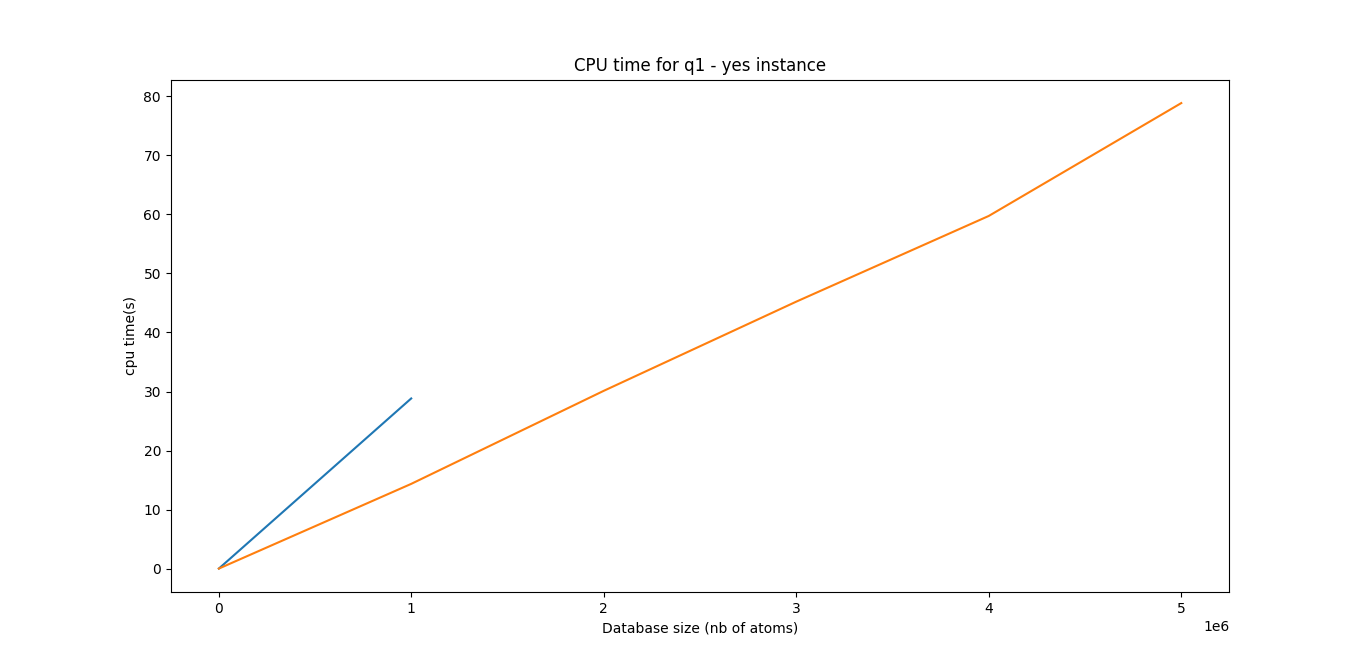
\includegraphics[width=0.6\textwidth]{time_q1_yesinstance.png}
\centering
\end{figure}

\begin{figure}[H]
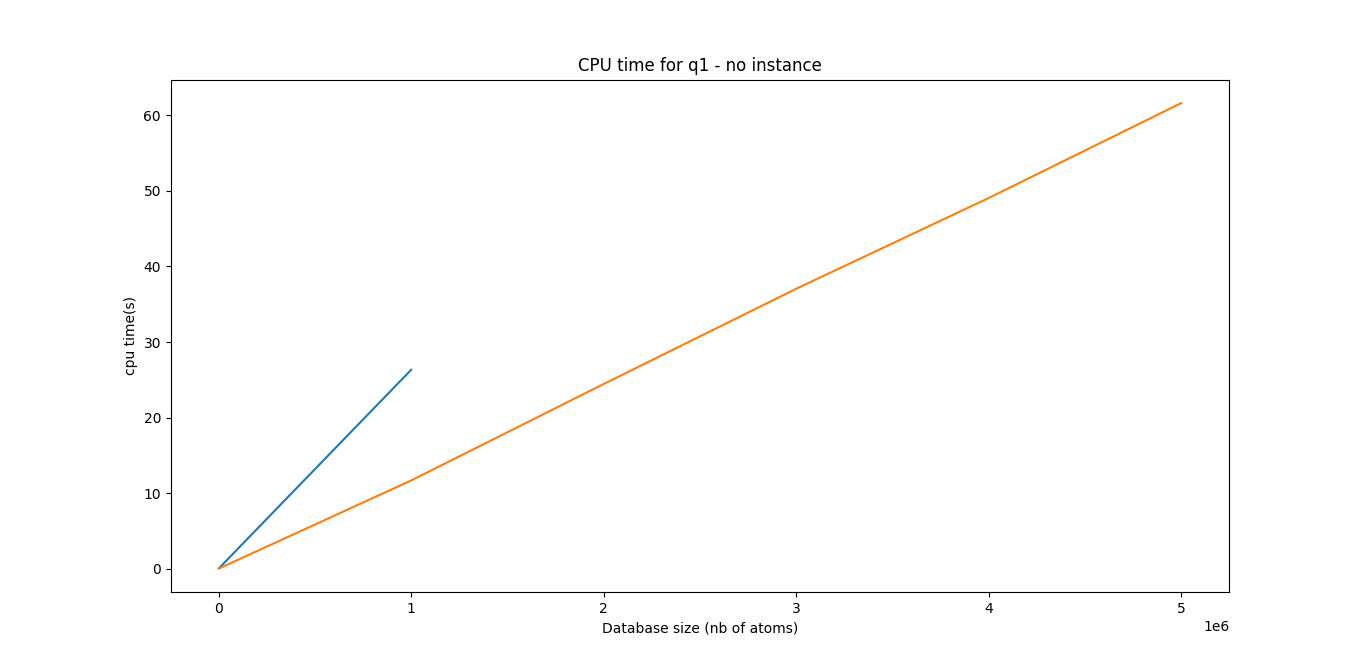
\includegraphics[width=0.6\textwidth]{time_q1_noinstance.png}
\centering
\end{figure}

\begin{figure}[H]
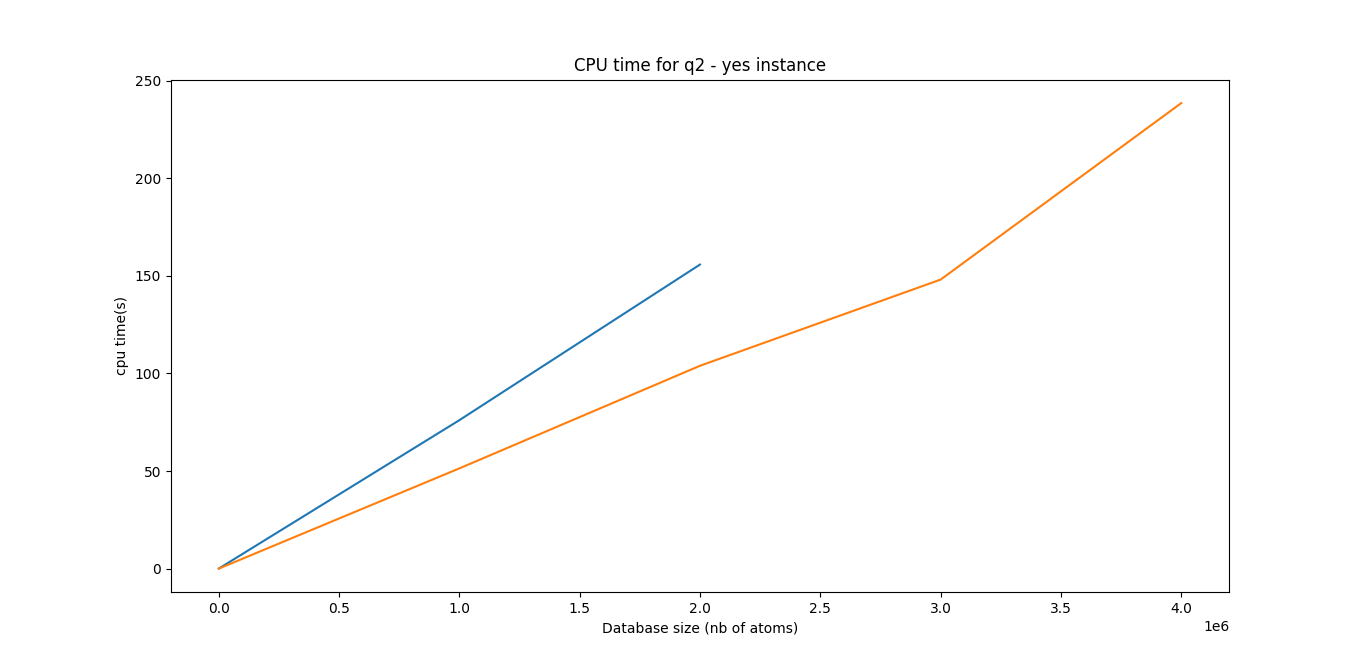
\includegraphics[width=0.6\textwidth]{time_q2_yesinstance.png}
\centering
\end{figure}

\begin{figure}[H]
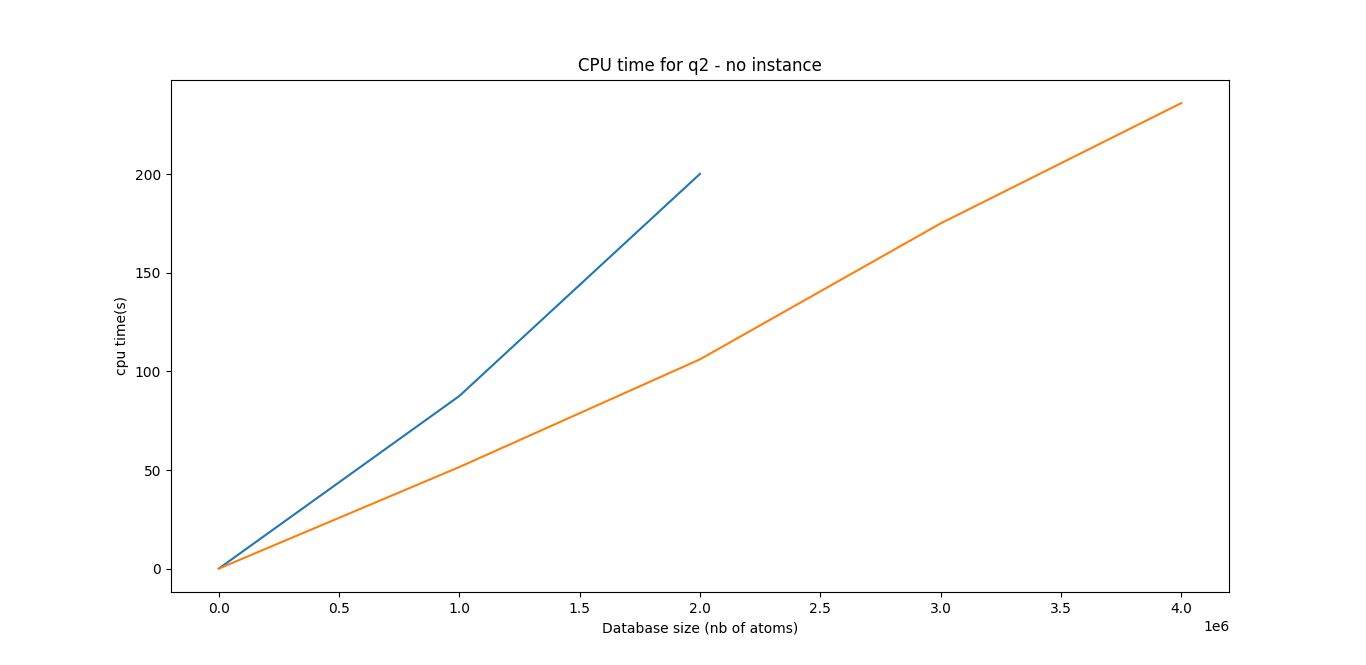
\includegraphics[width=0.6\textwidth]{time_q2_noinstance.png}
\centering
\end{figure}

\begin{figure}[H]
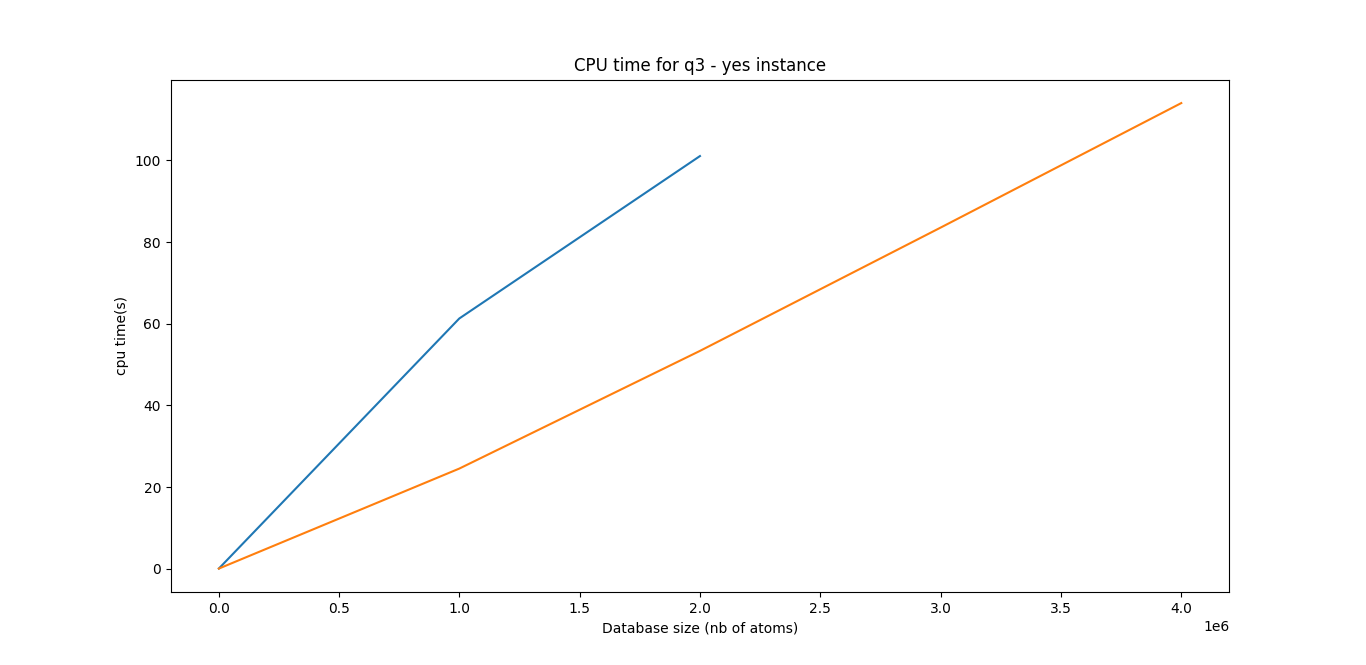
\includegraphics[width=0.6\textwidth]{time_q3_yesinstance.png}
\centering
\end{figure}

\begin{figure}[H]
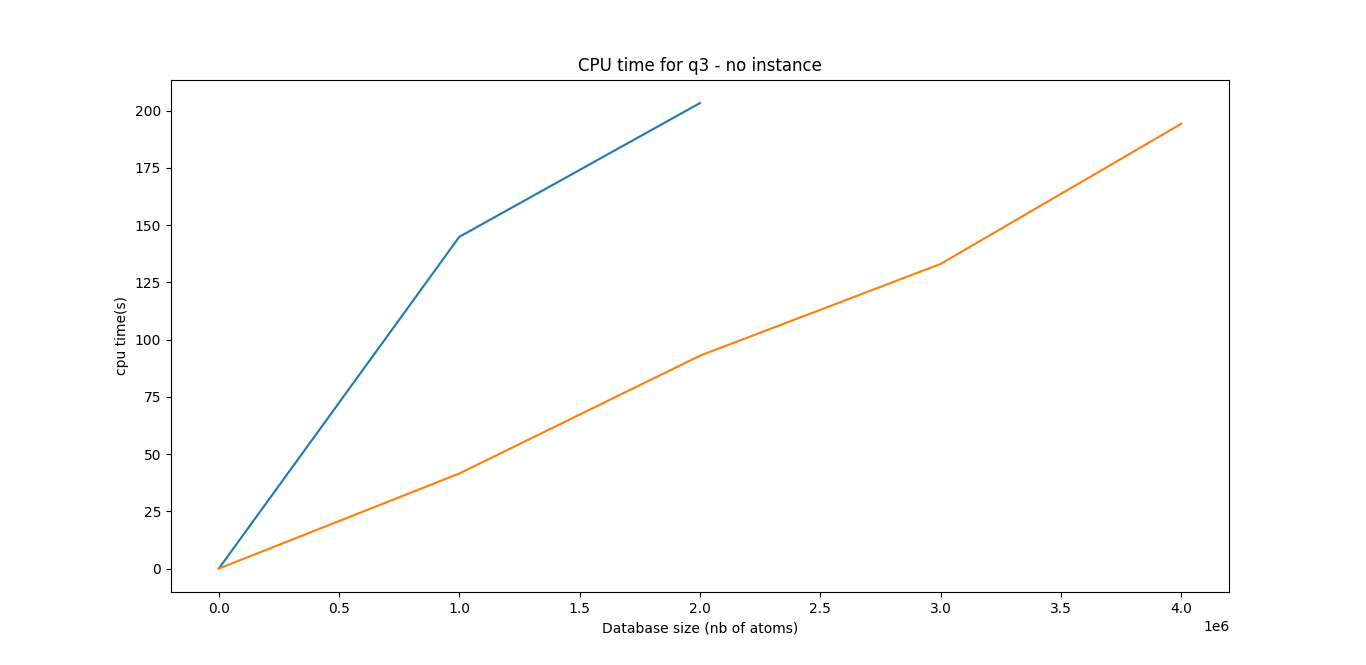
\includegraphics[width=0.6\textwidth]{time_q3_noinstance.png}
\centering
\end{figure}

We see that the fo rewriting leads to better results, in terms of cpu time, that the generate-and-test method.

\section{Conclusion}

We rewrited 7 first-order rewritable queries in ASP and showed that the fo rewriting are more efficient than a generate and test method. The first order rewriting consumes a lot less memory than the generate and test which cannot run on 8GB of RAM on a database containing 3 millions or more entries.
